\chapter{Introduction}

% \subsection*{Geodata \& Geodata computation}

The field of \ac{gis} concerns itself with the collection, processing, storage, and visualization of geodata. 
By doing do, we offer the world priceless information about the land we build on, the seas we traverse, the air we breath, and the climates we inhabit. 
This information is foundational for many applications, including environmental modelling, infrastructure, urban planning, navigation, the military, and agriculture.   

Central to this effort is the process of converting raw geodata into meaningful geo-information. 
Additionally, the effort often involves executing transformations or calculations on existing datasets. 
The term \ac{geocomputation}, or geodata processing, is used to represent all types of computations performed on geographical datasets. Anything from the calculation of the area of a region, to a \ac{crs} transformations, or converting a raster dataset into a vectorized dataset, can be regarded as geocomputation.
All applications of geo-informatics require some level of geocomputation, as the raw data gathered from surveyance seldom corresponds to the precise information we wish to discover about the earth.       
This makes geocomputation a cornerstone of the entire field of geo-informatics, and vital to all her applications.

However, geocomputation is no trivial exercise. The geometric nature of geocomputation, together with the sheer scope of geodata, and the variety in formats and quality make geocomputation both computationally intensive and difficult to operate. 

In an ideal world, the activity of geocomputation should be ergonomic: Operations must perform as fast as possible, and the effects of those operations must be both clear to the user, and reliable.
While researchers and developers have made considerable improvement over the last decades, the improvement of both geocomputation, and the activity of geocomputation, remains as relevant as ever before. 

In recent years, two promising developments regarding geocomputation are emerging:
Visual programming, and browser-based geocomputation. 
these two developments require further explanation, after which the subject and goal this thesis can be made clear.

\subsection*{Visual programming}

\begin{figure}
  \centering
  \graphicspath{{../../assets/images/background/geo-vpl/}}
  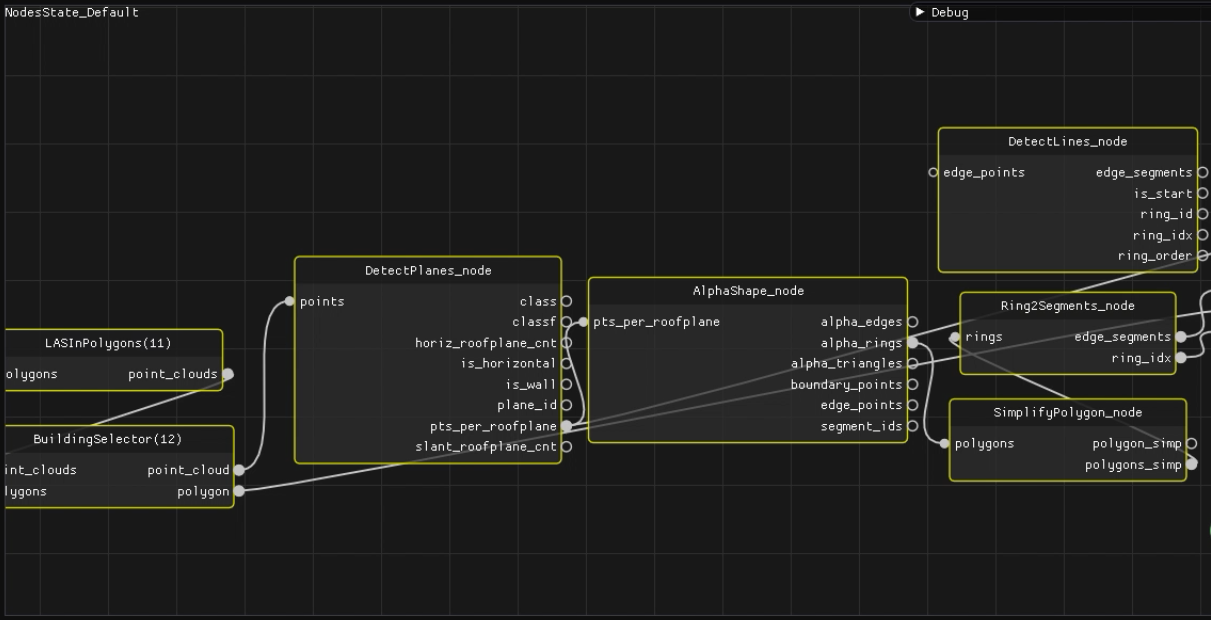
\includegraphics[width=\linewidth]{geoflow.png}
  \caption{Geoflow: A geocomputation VPL}
  \label{fig:1:geoflow}
\end{figure}

% \emph{what makes a vpl a 'new' development?}
\begin{note}
  TODO: this chapter should probably be rewritten to connect more to the current content of the thesis
\end{note}

The \ac{vpl} is still considered an ongoing development within the field of geocomputation, despite popular examples like FME (Source, TODO add picture). 
Especially in recent years, a push towards a more 'granular' \ac{vpl}s can be recognized: 
\ac{vpl}s offering more precise geocomputation on a smaller, more detailed level than the \ac{etl} tools of FME. 
As an example, McNeels's Grasshopper (SOURCE) is increasingly being used for spatial analyses of buildings and neighborhoods, like solar irradiation or heating demands (source). 
Meanwhile, GeoFlow (shown in \reffig{fig:1:geoflow}) was used to model the 3D envelope of a building based on a pointcloud, which was subsequently scaled up in the creation of the 3D BAG dataset (source).

Using a \ac{geo-vpl} for more detailed geocomputation is still relatively novel, and contains many open ended questions. That geocomputation in certain scenarios benefits from the interface offered by \ac{vpl}s like these is probably true, indicated by the number of prior studies on the topic (source, source, source), and the popularity of \ac{vpl}s used for geodata and geometry computation. The \emph{extend} to which \ac{vpl}s benefit detailed geocomputation, is still relatively unknown. 

\subsection*{Browser-based geocomputation}

\begin{figure}
  \centering
  \graphicspath{ {../../assets/images/background/geo-web/} }
  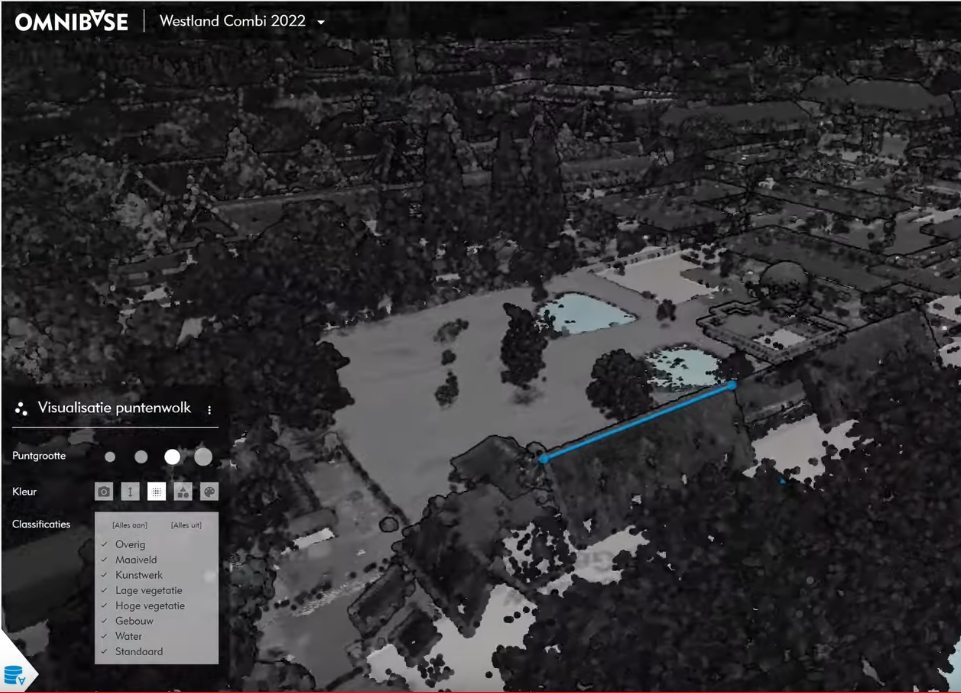
\includegraphics[width=250px]{omnibase.png}
  \caption{Omnibase: An example of browser-based geocomputation}
  \label{fig:1:omnibase}
\end{figure}

Browser-based \ac{geocomputation} is slowly gaining traction during the last decade \cite{kulawiak_analysis_2019, panidi_hybrid_2015, hamilton_client-side_2014}. 
Interactive geospatial data manipulation and online geospatial data processing techniques have been described as "current highly valuable trends in evolution of the Web mapping and Web GIS" \cite{panidi_hybrid_2015}. 
The central idea is to add browser-based geocomputation to web-mapping applications, allowing users not only to view geodata, but to analyze it, and even fine-tune the data to their own custom needs.
An example of this is the Omnibase application in \reffig{fig:1:omnibase}, used by Dutch municipalities to measure and map buildings and infrastructure.

Additionally, browser-based geocomputation, compared to native GUI or CLI geocomputation, allows geocomputation to be more \textbf{accessible} and \textbf{distributable}. 
Accessible, since geocomputation on the web requires no installment or configuration, 
and distributable, since the web is cross-platform by default, and poses many advantages for updating, sharing, and licensing applications. 
By performing these calculations in the browser rather than on a server, server resources can be spared, and customly computed geodata does not have to be resend to the user upon every computation request ([back up with sources from related works]).

However, Browser-based geocomputation also has many open-ended questions and challenges. 
The big catch is that browsers \& javascript are not ideal hosts for geocomputation. 
As an interpreted language, Javascript is slower and more imprecise compared to system-level languages like C++.
In addition, it has limited support regarding reading and writing files, and does not possess of a rich ecosystem of geocomputation libraries.  
Novel browser features like WebAssembly may pose a solution to some of these open questions, but this has not seen substantial research. 

%%%%%%%%%%%%%%%%%%%%%%%%%%%%%%%%%%%%%%%%%%%%%%%%%%%%%%%%%%%%%%%%%%%%%%%%%%%%%%%
%%%%%%%%%%%%%%%%%%%%%%%%%%%%%%%%%%%%%%%%%%%%%%%%%%%%%%%%%%%%%%%%%%%%%%%%%%%%%%%
%%%%%%%%%%%%%%%%%%%%%%%%%%%%%%%%%%%%%%%%%%%%%%%%%%%%%%%%%%%%%%%%%%%%%%%%%%%%%%%

% Note: this are all fragments and motivations. I'm leaving them here, don't
% be bothered by them, keep things concise, but if we need extra baggage, we 
% can get it from here. 

%%%%%%%%%%%%%%%%%%%%%%%%%%%%%%%%%%%%%%%%%%%%%%%%%%%%%%%%%%%%%%%%%%%%%%%%%%%%%%%
%%%%%%%%%%%%%%%%%%%%%%%%%%%%%%%%%%%%%%%%%%%%%%%%%%%%%%%%%%%%%%%%%%%%%%%%%%%%%%%
%%%%%%%%%%%%%%%%%%%%%%%%%%%%%%%%%%%%%%%%%%%%%%%%%%%%%%%%%%%%%%%%%%%%%%%%%%%%%%%

% This design of geofront contains several challenges. Browser-based geocomputation (BBGC) might not be as performant as back-end / native geocomputation \cite{panidi_hybrid_2015, hamilton_client-side_2014}, even with the usage of WebAssembly \cite{jangda_not_2019}. 
% Additionally, since current visual programming environments all fall short on at least one of the above features, the visual programming environment will have to be created from scratch.

% The cloud-native geospatial movement represents a significant opportunity and challenge to these VPL interfaces. The \textbf{opportunity} lies in the fact that a VPL interface is highly suitable as a 'configurator' or 'IDE' for cloud-computation. The promise of interactive, low-code automation matches the desire of most cloud native geocomputation providers to support users of different backgrounds, both programmers and non-programmers, both full GIS experts as well as non-experts (SOURCE: Modellab, SOURCE: Chris Holmes). A good example of this is the ModelLab VPL, found in Raster Foundry (SOURCE). This is also evident in the fact that existing VPL's like FME and Grasshopper have added proprietary cloud-computation features like FME Cloud (SOURCE) and ShapeDiver (SOURCE), respectively.

% <!-- HOWEVERRRRRRRRR -->
% However, the major \textbf{challenge} is that as of right now and despite these developments, popular VPL's fall short on a number of priorities and features required for cloud-native geospatial computation. 
% These shortcomings include their closed and proprietary nature, their distance from regular programming features and conventions (git version control, continuous integration), and the non-containerized, one to one relationship between the IDE application \& the cloud hosting platform. All of this hinders their suitability as general, cloud-computation configurers. 


% For a geocomputation method to match the 'cloud native geospatial movement'

% Currently, WebAssembly is the only way one can take a geocomputation function from an arbitrary source, and use it in both the browser and on a server. 
% We wish to discover if this has any practical use cases. 

% - "As massive datasets become more and move available, the availability of the \emph{means} to process and analyse these data becomes more and more relevant". 

% Despite these advantages, open, accessible vpl's are often unavailable. 
% - Expensive, proprietary environments 
% - Require specific plugins in order to utilize open, industry standard geocomputation libraries
% - Not FAIR geocomputation

%%%%%%%%%%%%%%%%%%%%%%%%%%%%%%%%%%%%%%%%%%%%%%%%%%%%%%%%%%%%%%%%%%%%%%%%%%%%%%%

% This thesis explores if these in-between processing steps could also be performed within a web application.  

% This way, geodata processing applications could profit from the ease of accessibility and maintainability granted by the web as a platform.  

% <!-- More Why of web GIS and web-geocomputation: 
% - making the geoweb more feature-rich
% - allowing quick demonstration (wapm)
% - allowing easy access (overleaf)

% ## Motivation
% Under normal circumstances, Web applications within the field of geo-informatics are mostly used for the first and final stages of a common geodata process: Retrieval and visualization. 
% The processing stages in-between are almost always performed on the desktop using environments like QGIS or ArcGIS, or by writing and using CLI tools. 

% <!-- At the same time, a need arrises -->

%%%%%%%%%%%%%%%%%%%%%%%%%%%%%%%%%%%%%%%%%%%%%%%%%%%%%%%%%%%%%%%%%%%%%%%%%%%%%%%

% Under normal circumstances, Web applications within the field of geo-informatics are mostly used for the first and final stages of a common geodata process.  
% (
% If one wishes to retrieve geodata, web portals are used to discover the required datasets. After this, the OGC Web Services are often utilized to download and truly access this geodata. 

% This geodata is then processed locally, using QGIS, ArcGIS, command line tools, or any other 

% and at the end Tools like Leaflet and Celcium have been created to visualize the earth in both 2D and 3D , and tools like d3.js can produce interactive graphs to supplement these web pages. 

% There is, however, more to the web than just visualization. Due to 
% )
% This thesis asks the question if the web could do more than just visualization. 

% By creating the use-case application GeoFront, we ask the question if a modern web browser, and the current state of the client-side web technologies are capable of facilitating  

%%%%%%%%%%%%%%%%%%%%%%%%%%%%%%%%%%%%%%%%%%%%%%%%%%%%%%%%%%%%%%%%%%%%%%%%%%%%%%%

\section{Problem Statement}
% \begin{note}
%   TODO: make both of these presuppositions clear
%   1. Combining a geo-vpl and bbg is useful. It is valuable to figure out if it can be done properly
%   2. properly -> utilization of existing, native geocomputation libraries within a VP environment is key to making a geo-web-vpl succeed. 
% \end{note}

The proven usefulness of a vpl for geodata computation, together with the theorized potential of browser-based geocomputation, lead to the idea of a \ac{geo-web-vpl}. 
regrettably, this topic has seen little to no prior study, even though a \ac{geo-web-vpl} could be the next step in the pursuit of making the activity of geocomputation more clear and reliable.
The activity of geocomputation could benefit from the experimentation and debugability advantages of a \ac{vpl}, combined with the accessibility and distribution advantages of a web application.
This format might even yield completely unique benefits.
% making geocomputation more appealing for a larger group of end-users
% , by means of a "1 + 1 = 3" line of reasoning.
However, since only a very small number of geo-web-vpls exist, there are not enough examples to definitively proof or test these aspects. 

Additionally, prior studies give an indication to certain disconnects between the fields of geo-VPLs and web-GIS. 
This is further explained in \refchap{chap:related}.
Multiple existing geo-VPLs are encountered which cannot be used in a browser, while  many web-based VPLs are unable to support existing, native geocomputation functionalities. 
From this, it can be concluded that bridging this gap is vital in making any geo-web-vpl succeed. 

%%%%%%%%%%%%%%%%%%%%%%%%%%%%%%%%%%%%%%%%%%%%%%%%%%%%%%%%%%%%%%%%%%%%%%%%%%%%%%%

\section{Research Objective}

This study seeks to close the gap between geo-VPLs and browser-based geocomputation by designing, implementing, and evaluating a new prototype \ac{geo-web-vpl}.
The study starts from the presupposition that proper utilization of existing, native geocomputation libraries within a visual programming environment is key to making a geo-web-vpl succeed. 
Overcoming this technical challenge is the focal point of this study. 

\section{Research Questions}
Based on this objective, the research question is formulated as follows: 
\begin{itemize}[ ]
  \item \myMainRQ
\end{itemize}

\subsection*{Supporting Questions}
The following supporting questions are defined to aid in answering the main question.
These are based upon various components of the main problem statements, further explained in \refchap{chap:methodology}
\begin{itemize}[-]
  \item \mySubRQOne
  \item \mySubRQTwo
  \item \mySubRQThree
  \item \mySubRQFour
\end{itemize}
In order to obtain answers to these questions, a literature review is performed,
a prototypical software application is developed, 
and this application is tested and accessed on various aspects.

\newpage
\section{Scope}
The scope of this thesis is cornered in the following six ways: 

\subsection*{Only frontend geocomputation}
This study excludes any \emph {backend} based geocomputation.
A web application \textit{could} be used to orchestrate geocomputation web-services, which could also deliver a form of browser-based geocomputation to end-users. 
However, for the scope of this thesis, we limit ourselves to purely client-side solutions, with calculations literally happening within the clients browser. 
This is also why this study excludes the OGC standard of the \ac{wps} \cite{ogc_web_2015}.

Adding backend-based geocomputation to a geo-web-VPL would be an excellent follow-up investigation to this study. 
Future work could research the possibility of utilizing a hybrid strategy of both client-side and server-side geocomputation, following in the footsteps of \cite{panidi_hybrid_2015}. 

\subsection*{No Usability Comparison} % 
While accessibility / usability is a motivation of the development of a \ac{vpl}, and while usability will be analyzed to a limited extend, no claims will be made that this method of geocomputation is \emph{more} usable as opposed to existing geocomputation methods. This research attempts to solve practical inhibitions in order to discover whether or not browser-based, vpl-based geocomputation is \emph{a} viable, usable option. If it turns out that this method is viable enough technically, future research will be needed to definitively proof \emph{how} usable it is compared to all other existing methods.  

% This paper seeks to first close this gap, limiting itself to overcoming the technical and design boundaries in the pursuit of practical client-side geocomputation.

Similarly, a survey analyzing how users experience browser-based geocomputation in comparison to native geocomputation must also be left to subsequent research. While this would be insightful, client-side geocomputation is too new to make a balanced comparison. Native environments like QGIS, FME or ArcGIS simply have a twenty year lead in research and development. 

% While the research restrains itself from empirically measuring an aspect as nebulous as 'accessibility', it does demonstrate ...


% It is my goal to introduce this as a new geocomputation option, and to name the advantages and disadvantages we can be sure of. An actual comparison of client-side vs native geocomputation is something different. 

\subsection*{Only WebAssembly-based containerization}
This thesis examines a WebAssembly-based approach to containerization and distribution of geocomputation functionalities. 
Containerization using Docker is also possible for server-side applications, but is not (easily) usable within a browser. 
For this reason, Docker-based containerization is left out of this studies' examination. 
And to clarify: Docker and WebAssembly are not mutually exclusive models, and could be used in conjunction on servers or native environments. 

\subsection*{Mostly Point Cloud/ DTM focussed geocomputation}
We are also required to concentrate the scope of 'geocomputation', which is a sizable phenomenon.
The term is generally used to cover all operations on geodata, from rasters, tabular datasets, highly structured datasets such as the CityJSON or IndoorGML, and point clouds. 
Due to time limitations, we are forced to focus on particular type of geocomputation.
3D-based geocomputation is chosen, with a particular focus on pointclouds and DTMs. 
The hypothesis is that these types of data may fit the small-scale geocomputation of a 'geo-web-vpl' well due to the local optimality quality of many DTM procedures (Such as the \ac{dt}), 

\subsection*{Assumption: a '\ac{geo-web-vpl}' is a normal Geometry VPL able to handle geodata}
For the scope of this thesis, we assume a Web-VPL for geocomputation is practically the same as a web-VPL for generic geometry processing.
Examples of "Geometry VPLs" are Blender's Geometry Nodes, Houdini, GeoFlow, and Grasshopper.
More on this in chapter \refsec{sec:related-geovpl}.

A geo-web-vpl differs only in the fact that it supports additional geodata types, and offers functionalities specific to processing those types.  
This assumption is safe to make since a 'geo-web-vpl' will \emph{at the very least} require the same features as a 'normal' geometry VPL, due to their common dependency on the field of computer graphics and computational geometry.

Still, in reality, a lot of differences and nuances exist between the field of geocomputation and the field of procedural modelling. 
However, due to time limitations, these concerns are left to future research.
% these concerns will only be picked up at the final discussion, found at \refsec{sec:discussion}.
 
\subsection*{Only core browser features}
Lastly, the implementation of the geo-web-vpl will limit itself to core browser features, keeping dependencies at a minimum, in an attempt to generalize the results of the study.
If the study would use very specific web frameworks and technologies to solve key issues, questions might arise if the results of the study counts in general for browser-based geocomputation or geo-VPLs, or if they only count in this very specific scenario. 
"Core browser features" is defined in \refsec{sec:method-one}.

\newpage
\section{Reading Guide}
The remainder of this study is structured as follows:

\begin{itemize}[ ]
  \item \refchap{chap:background}, Background, provides an overview of the theoretical background that is used in the rest of this study.
  
  \item \refchap{chap:related}, Related Work, provides a review of studies comparable to this one.

  \item \refchap{chap:methodology}, Methodology, explains precisely in what way the research-questions will be answered, and shows how this relates to the background and related works chapters. 

  \item \refchap{chap:implementation}, Implementation, presents the implementation of the methodology.
  In addition, the main design decisions are described and justified in this part of the study.
  
  \item \refchap{chap:analyses} analyses the results from this implementation in the various ways described by the methodology.
  
  \item And finally, \refchap{chap:conclusion}: Conclusion \& Discussion, concludes to which extend the study was able to satisfy the main research question, and discusses unaddressed aspects of the thesis.
  It also includes the envisioned future works and a reflection on the quality of the study.

\end{itemize}